\subsection{Discovering morphological categories}
\label{sec:categories}

Besides being sensitive, to some extent, to word boundaries, does
the CNLM also store linguistic properties of words, such as their part
of speech and number? These experiments focus on German and
Italian, as it's harder to design reliable test sets for
morphologically impoverished English.

\paragraph{Word classes (nouns vs.~verbs)}

We sampled 500 verbs and 500 nouns from the Wikipedia training sets,
requiring that they end in -\emph{en} (German) or -\emph{re} (Italian)
(so that models can't rely on the affix for classification), and that
they are unambiguously tagged in the corpus. %The first constraint sets
% the bar higher for methods relying on surface cues, as all verbs and
% nouns share the same endings.
We randomly selected 20 training
examples (10 nouns and 10 verbs), and tested on the
remaining items.  We repeated the experiment 100 times to control
for random train-test split variation. We recorded the final
hidden state of a pre-trained CNLM after reading a word, without
context, and trained a logistic noun-verb classifier on these
representations.

As a baseline, we used a character-level LSTM autoencoder trained to
reconstruct words in isolation.  The hidden state of the autoencoder
should capture relevant orthographic features.  We further considered
word embeddings from the output layer of the WordNLM, reporting its test accuracy both when OOV words are ignored and when they are randomly classified.
%\textbf{This needs to be further discussed: can you compute  performance with random guess for OOV words?}

Results are shown in Table~\ref{tab:pos-results}.  All language models
outperform the autoencoders, showing that they learned categories
based on broader distributional evidence, not just typical strings
cuing nouns and verbs. Moreover, the LSTM CNLM outperforms the RNN,
probably because it can track broader contexts. Not surprisingly, the
word-based model fares better, but the gap, especially in Italian, is
rather narrow, and there is a strong negative impact of OOV words. % Figure~\ref{fig:pos-induction} shows how German performance evolves as the training set grows from 2 to 100 examples (Italian results are qualitatively identical). The CNLMs already distinguish the categories well with small training sets, while the autoencoder does not catch up even with 100 training examples per category.

\begin{table}[t]
%  \begin{small}
\footnotesize
    \begin{center}
      \begin{tabular}{l|l|l}
        &\emph{German}&\emph{Italian}\\
        \hline
        LSTM & 89.0 ($\pm$ 0.14) & 95.0 ($\pm$ 0.10) \\
        RNN & 82.0 ($\pm$ 0.64) & 91.9 ($\pm$ 0.24) \\
        Autoencoder & 65.1 ($\pm$ 0.22) & 82.8 ($\pm$ 0.26) \\
        WordNLM & 97.4 ($\pm$ 0.05) & 96.0 ($\pm$ 0.06) \\
        WordNLM (all words) & 53.5 ($\pm$ 0.18)  & 62.5 ($\pm$ 0.26) \\
      \end{tabular}
    \end{center}
 % \end{small}
  \caption{\label{tab:pos-results} Word class accuracy, with standard errors.} % (20 training examples)
\end{table}


% \begin{figure}
% 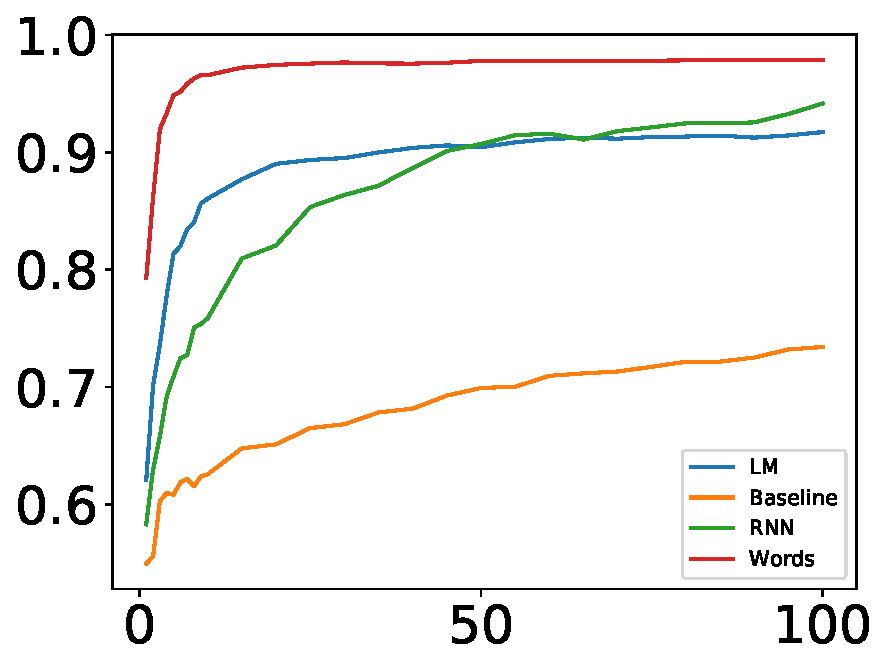
\includegraphics[width=0.48\textwidth]{figures/german_pos_nouns_verbs.pdf}
% 	\caption{Word class accuracy as a function of training examples (German). }\label{fig:pos-induction}
% 	% \textbf{Please rename LM LSTM, Baseline Autoencoder and Words WordNLM}
% \end{figure}





\paragraph{Number}
We turn next to number, a more granular morphological feature. We
study German as it possesses nominal classes that form plural
through different morphological processes. We train a number
classifier on a subset of these classes, and test on the others. If a
model generalizes correctly, it means that it is sensitive to number
as an abstract feature, independently of its surface expression.

We extracted plural nouns from the German UD
treebank \cite{de2006generating,mcdonald2013universal}.  We selected
nouns with plurals in -\emph{n}, -\emph{s}, or -\emph{e} to train the classifier (e.g., \emph{Geschichte-n} `stories'), and tested on plurals formed with
-\emph{r} or through vowel change (\emph{Umlaut}, e.g., \emph{T{\"o}chter} for singular \emph{Tochter} `daughter').
%\textbf{Add one
%  example from training, one from testing.}

For the training set, we randomly selected 15 singulars and plurals
from each training class.  As plural suffixes make words longer, we
sampled singulars and
plurals %used rejection sampling \textbf{(cite something?)}
from a single distribution over lengths, to ensure that their lengths
were approximately matched.  For the test set, we selected all plurals
in -\emph{r} (127) or Umlaut (38), with their respective
singulars. %\textbf{(how many?)}.
We also used all remaining plurals ending in -\emph{n} (1467), -\emph{s} (98) and -\emph{e} (832) as in-domain test data.
%\textbf{Need information on the test set for the training classes.}
To control for the impact of training sample selection, we
report accuracies averaged over 200 repetitions.  We extract word
representations as above, and we compare to an autoencoder and
embeddings from the WordNLM.
As before, we report results ignoring OOV words, and with random classification for OOV words.
%, excluding OOVs when testing the latter.
Results are summarized in Table \ref{tab:number-results}.

\begin{table}[t]
	\footnotesize
  \begin{center}
    \begin{tabular}{@{\hspace{0.5em}}l@{\hspace{0.5em}}|@{\hspace{0.5em}}c@{\hspace{0.5em}}|@{\hspace{0.5em}}l@{\hspace{0.7em}}l@{\hspace{0.5em}}}
      &train classes&\multicolumn{2}{c}{test classes}\\
      &\emph{-n/-s/-e}&\multicolumn{1}{c}{\emph{-r}}&\multicolumn{1}{c}{\emph{Umlaut}}\\      \hline
	    LSTM& 77.9 ($\pm$ 0.8) & 88.2 ($\pm$ 0.3) & 52.8 ($\pm$ 0.6) \\
	    RNN& 70.3 ($\pm$ 0.9) & 81.3 ($\pm$ 0.7) & 53.3 ($\pm$ 0.6)\\
	    Autoencoder& 64.0 ($\pm$ 1.0) & 73.8 ($\pm$ 0.6) & 59.2 ($\pm$ 0.5)\\
	    WordNLM& 97.8 ($\pm$ 0.3) & 86.6 ($\pm$ 0.2) & 96.7 ($\pm$ 0.2)  \\ 
	    WordNLM (A) & 82.1 ($\pm$ 0.1) & 73.1 ($\pm$ 0.1) & 77.6 ($\pm$ 0.1)  \\ 
    \end{tabular}
  \end{center}
	\caption{\label{tab:number-results} German number classification accuracy, with standard errors computed from 200 runs.}
\end{table}


% \begin{table}[t]
% 	\footnotesize
%   \begin{center}
%     \begin{tabular}{l|c|l|lllllll}
%       &train classes&\multicolumn{2}{c}{test classes}\\
%       &\emph{-n/-s/-e}&\emph{-r}&\emph{Umlaut}\\      \hline
% 	    LSTM& 77.9 ($\pm$ 0.8) & \textbf{88.2} ($\pm$ 0.3) & 52.8 ($\pm$ 0.6) \\
% 	    RNN& 70.3 ($\pm$ 0.9) & 81.3 ($\pm$ 0.7) & 53.3 ($\pm$ 0.6)\\
% 	    Autoencoder& 64.0 ($\pm$ 1.0) & 73.8 ($\pm$ 0.6) & 59.2 ($\pm$ 0.5)\\
% 	    WordNLM& \textbf{97.8 ($\pm$ 0.3)} & 86.6 ($\pm$ 0.2) & \textbf{96.7} ($\pm$ 0.2)  \\ % when including OOVs: 81.0/83.8/81.5 & 72.9 & 77.6\\
%     \end{tabular}
%   \end{center}
% 	\caption{\label{tab:number-results} German number classification accuracy, with standard errors computed from 200 runs.}
% \end{table}



%\begin{table}[t]
%  \begin{center}
%    \begin{tabular}{l|l|l|lllllll}
%      &train classes&\multicolumn{2}{|c}{test classes}\\
%      &\emph{-n/-s/-e}&\emph{-r}&\emph{Umlaut}\\      \hline
%	    LSTM& 77.9 ($\pm$ 0.76) & \textbf{88.2} ($\pm$ 0.32) & 52.8 ($\pm$ 0.57) \\
%	    RNN& 70.3 ($\pm$ 0.88) & 81.3 ($\pm$ 0.72) & 53.3 ($\pm$ 0.64)\\
%	    Autoencoder& 64.0 ($\pm$ 0.96) & 73.8 ($\pm$ 0.61) & 59.2 ($\pm$ 0.47)\\
%	    WordNLM& \textbf{97.8 ($\pm$ 0.26)} & 86.6 ($\pm$ 0.15) & \textbf{96.7} ($\pm$ 0.19)  \\ % when including OOVs: 81.0/83.8/81.5 & 72.9 & 77.6\\
%    \end{tabular}
%  \end{center}
%	\caption{\label{tab:number-results} German number classification accuracy, with standard errors computed from 200 runs.}
%\end{table}
%



%\begin{table*}[t]
%  \begin{center}
%    \begin{tabular}{l|l|l|l}
%      &\multicolumn{1}{c}{train classes}&\multicolumn{2}{|c}{test classes}\\
%      &\multicolumn{1}{c}{\emph{-n/-s/-e}}&\emph{-r}&\emph{Umlaut}\\      \hline
%      LSTM& 82.1 ($\pm$ 0.74)/68.0 ($\pm$ 0.87)/83.7 ($\pm$ 0.68)  & \textbf{88.2} ($\pm$ 0.32) & 52.8 ($\pm$ 0.57) \\
%      RNN& 77.6 ($\pm$ 0.81)/60.0 ($\pm$ 0.94)/73.4 ($\pm$ 0.89) & 81.3 ($\pm$ 0.72) & 53.3 ($\pm$ 0.64)\\
%      Autoencoder& 73.2 ($\pm$ 0.97)/54.5 ($\pm$ 0.93)/64.4 ($\pm$ 0.99) & 73.8 ($\pm$ 0.61) & 59.2 ($\pm$ 0.47)\\
%	    WordNLM& \textbf{97.1 ($\pm$ 0.31)/97.9 ($\pm$ 0.27)/98.5 ($\pm$ 0.20)} & 86.6 ($\pm$ 0.15) & \textbf{96.7} ($\pm$ 0.19)  \\ % when including OOVs: 81.0/83.8/81.5 & 72.9 & 77.6\\
%    \end{tabular}
%  \end{center}
%	\caption{\label{tab:number-results} German number classification accuracy, with standard errors computed from 200 runs.}
%\end{table*}

%python char-lm-ud-stationary-separate-bidir-with-spaces-probe-baseline-prediction-wiki-plurals-2-tests-RNN.py  --batchSize 256 --char_dropout_prob 0.01 --char_embedding_size 50 --char_noise_prob 0.0 --hidden_dim 2048 --language german --layer_num 2 --learning_rate 0.1 --nonlinearity tanh --load-from wiki-german-nospaces-bptt-rnn-237671415 --sequence_length 30 --weight_dropout_hidden 0.0 --weight_dropout_in 0.0
%python char-lm-ud-stationary-separate-bidir-with-spaces-probe-baseline-prediction-wiki-plurals-2-tests-words.py  --language german --batchSize 128 --char_embedding_size 200 --hidden_dim 1024 --layer_num 2 --weight_dropout_in 0.1 --weight_dropout_hidden 0.35 --char_dropout_prob 0.0 --char_noise_prob 0.01 --learning_rate 0.2 --load-from wiki-german-nospaces-bptt-words-966024846


The classifier based on word embeddings is the most successful,
confirming that the latter reliably encode number
\cite{Mikolov:etal:2013a}.  CNLM encodings outperform the autoencoder
on plurals formed with suffixes, indicating some capability to detect
number beyond orthographic cues.  For -\emph{r} plurals, the CNLM LSTM
even outperforms the WordNLM.  In contrast, the CNLMs do not
generalize to Umlaut plurals, where they are virtually at chance level,
and \emph{worse} than the autoencoder. Evidently, CNLM number encoding
is not abstract enough to generalize across very different surface
morphological processes (adding a suffix vs.~changing the root vowel).
